\documentclass[aspectratio=169,11pt]{beamer}
\usepackage{teaching_slides}



% \usepackage{slashbox}
\title{Lecture 6b: Logit Probit}
\author{Chris Conlon }
\institute{NYU Stern }
\date{\today}

\newcommand{\fp}{\frame[plain]}


\begin{document}
\maketitle

\begin{frame}
\frametitle{Binary Choice: Overview}
Many problems we are interested in look at discrete rather than continuous outcomes:
\begin{itemize}
\item Entering a Market/Opening a Store
\item Working or a not
\item Being married or not
\item Exporting to another country or not
\item Going to college or not
\item Smoking or not
\item etc.
\end{itemize}
\end{frame}

\begin{frame}
\frametitle{Simplest Example: Flipping a Coin}
Suppose we flip a coin which is yields heads ($Y=1$) and tails ($Y=0$). We want to estimate the probability $p$ of heads:
\begin{align*}
Y_i =
\begin{cases}
1 \mbox{ with probability } p \\
0 \mbox{ with probability } 1-p
\end{cases}
\end{align*}
We see some data $Y_1,\ldots,Y_N$ which are (i.i.d.)\\
\vspace{0.2cm}
We know that $Y_i \sim Bernoulli(p)$.
\end{frame}


\begin{frame}{Simplest Example: Flipping a Coin}
We can write the likelihood of $N$ Bernoulli trials as a Binomial: 
$$\Pr(Y_1 = y_1, Y_2=y_2,\ldots,Y _N=y_N )  =  f(y_1,y_2,\ldots,y_N | p ) $$
\begin{align*}
&= \prod_{i=1}^N p^{y_i} (1-p)^{1-y_i}\\
&= p^{\sum_{i=1}^N y_i} (1-p)^{N-\sum{i=1}^N y_i}
\end{align*}
And then take logs to get the \alert{log likelihood}:
\begin{align*}
\ln  f(y_1,y_2,\ldots,y_N | p )  &= \left( \sum_{i=1}^N y_i \right)  \ln p  + \left(N-\sum_{i=1}^N y_i \right)  (1-p)
\end{align*}
\end{frame}

\begin{frame}{Simplest Example: Flipping a Coin}
Differentiate the log-likelihood to find the maximum:
\begin{align*}
\ln  f(y_1,y_2,\ldots,y_N | p )  &= \left( \sum_{i=1}^N y_i \right)  \ln p  + \left(N-\sum_{i=1}^N y_i \right)  \ln(1-p)\\
\rightarrow 0&= \frac{1}{\hat{p}}  \left( \sum_{i=1}^N y_i \right) + \frac{-1}{1-\hat{p}}   \left(N-\sum_{i=1}^N y_i \right) \\
 \frac{\hat{p}}{1-\hat{p}} &= \frac{\sum_{i=1}^N y_i }{N- \sum_{i=1}^N y_i } = \frac{\overline{Y}}{1-\overline{Y}} \\
\hat{p}^{MLE} &= \overline{Y}
\end{align*}
That was a lot of work to get the obvious answer: \alert{fraction of heads}.
\end{frame}

\begin{frame}{More Complicated Example: Adding Covariates}
We probably are interested in more complicated cases where $p$ is not the same for all observations but rather $p(X)$ depends on some covariates. Here is an example from the Boston HMDA Dataset:
\begin{itemize}
\item 2380 observations from 1990 in the greater Boston area.
\item Data on: individual Characteristics, Property Characteristics, Loan Denial/Acceptance (1/0).
\item Mortgage Application process circa 1990-1991:
\begin{itemize}
\item Go to bank
\item Fill out an application (personal+financial info)
\item Meet with loan officer
\item Loan officer makes decision
\begin{itemize}
\item Legally in race blind way (discrimination is illegal but rampant)
\item Wants to maximize profits (ie: loan to people who don't end up defeaulting!)
\end{itemize}
\end{itemize}
\end{itemize}
\end{frame}


\begin{frame}{Loan Officer's Decision}
Financial Variables:
\begin{itemize}
\item $P/I$ ratio
\item housing expense to income ratio
\item loan-to-value ratio
\item personal credit history (FICO score, etc.)
\item Probably some nonlinearity:
\begin{itemize}
\item Very high $LTV > 80\%$ or $>95\%$ is a bad sign (strategic defaults?)
\item Credit Score Thresholds
\end{itemize}
\end{itemize}
\end{frame}


\begin{frame}{Loan Officer's Decision}
Goal $\Pr(Deny=1 | black, X)$\\

\begin{itemize}
\item Lots of potential \alert{omitted variables} which are correlated with race
\begin{itemize}
\item Wealth, type of employment
\item family status
\item credit history
\item zip code of property
\end{itemize}
\item Many \alert{redlining} cases hinge on whether or not black applicants were treated in a discriminatory way.
\end{itemize}
\end{frame}

\begin{frame}
\begin{center}
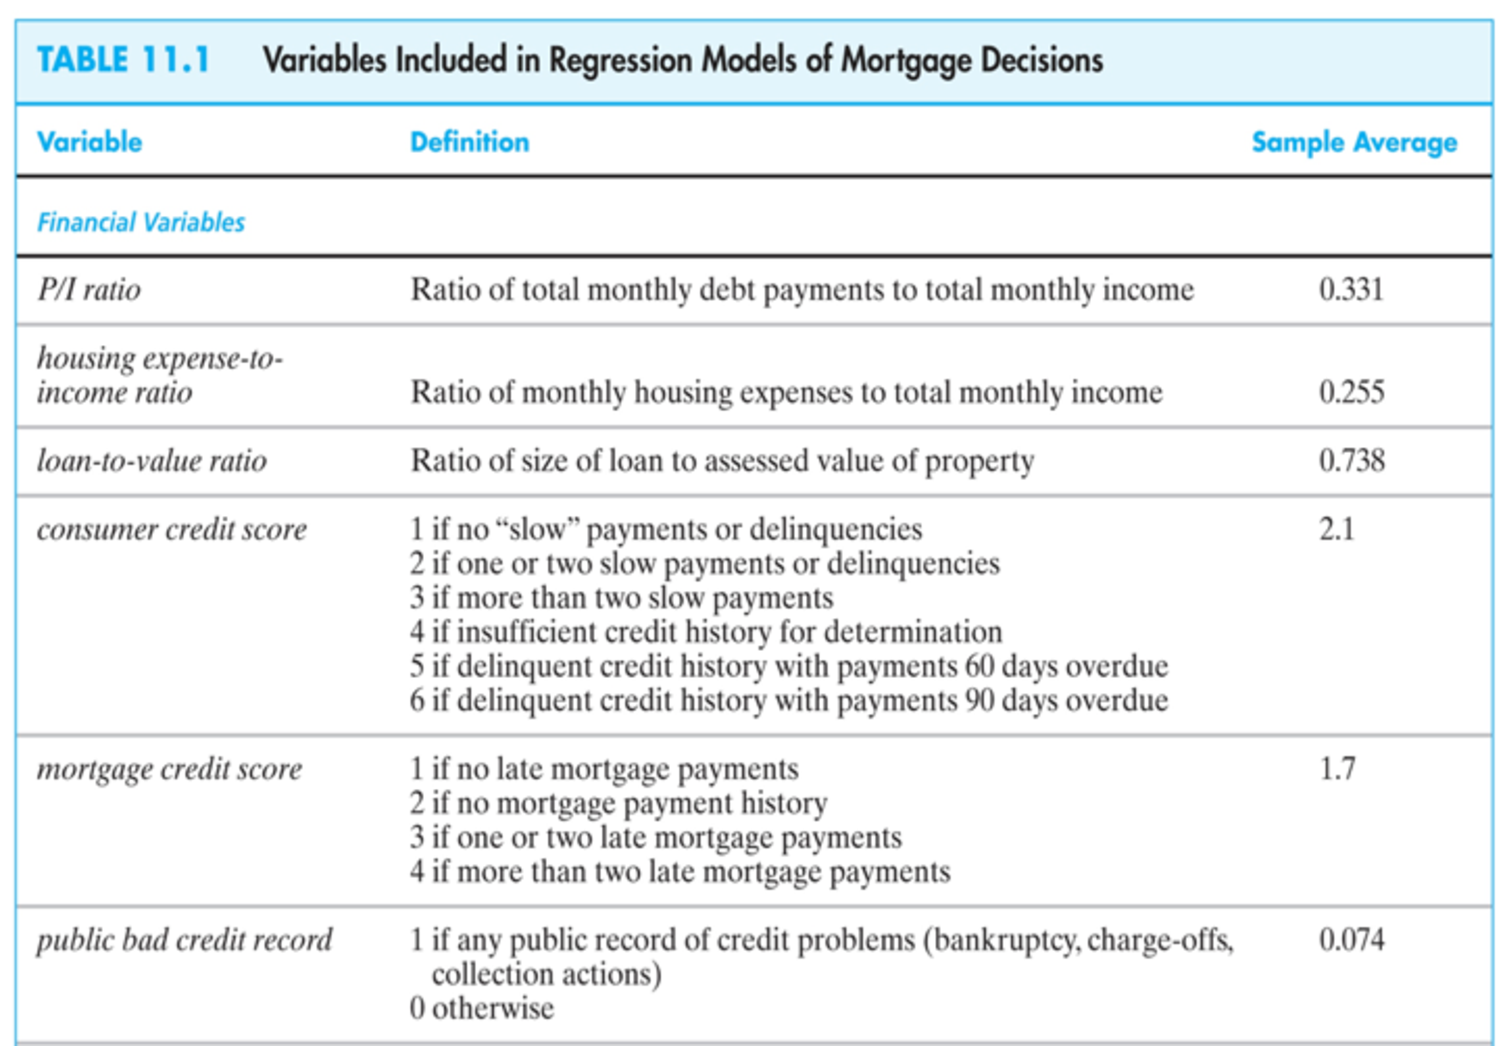
\includegraphics[width=3.25in]{resources/hmda1.pdf}\\
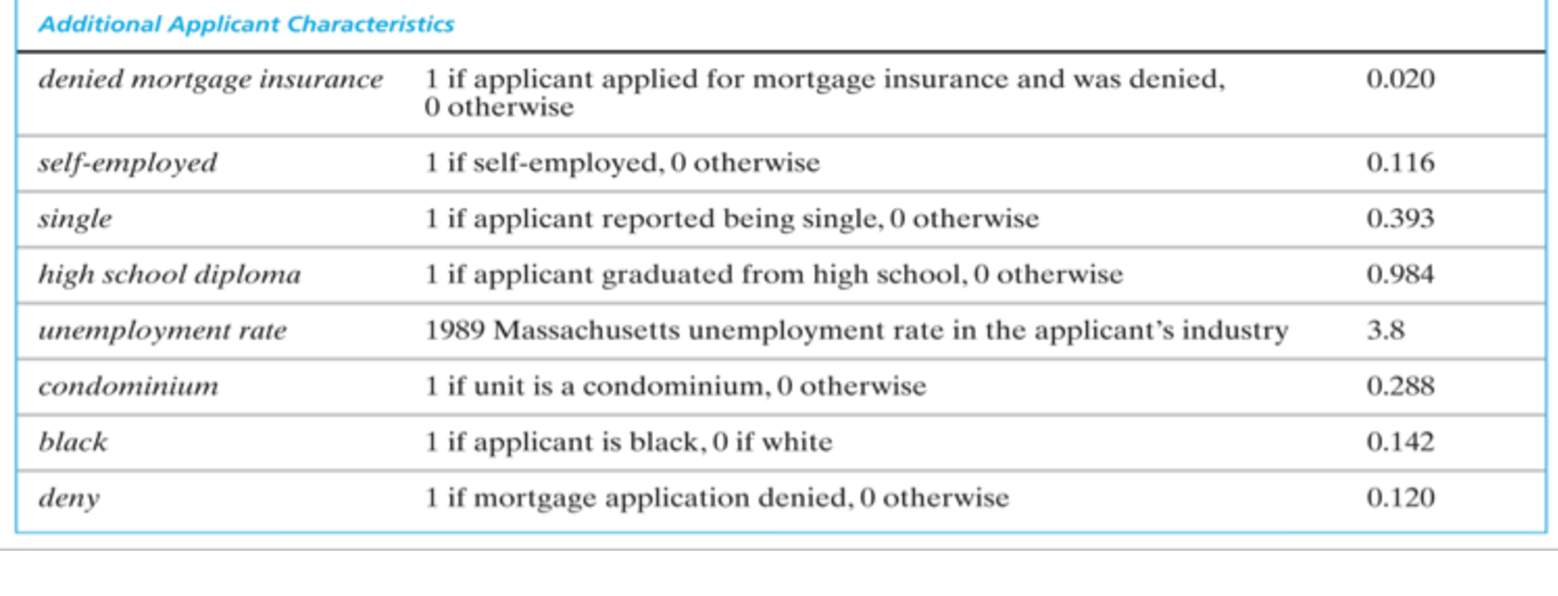
\includegraphics[width=3.25in]{resources/hmda2.pdf}
\end{center}
\end{frame}


\begin{frame}{Linear Probability Model}
First thing we might try is OLS
\begin{align*}
Y_i  = \beta_0 + \beta_1 X_i + \varepsilon_i
\end{align*}
\begin{itemize}
\item What does $\beta_1$ mean when $Y$ is binary? Is $\beta_1  = \frac{\Delta Y}{\Delta X}$?
\item What does the line $\beta_0 + \beta_1 X$ when $Y$ is binary?
\item What does the predicted value $\hat{Y}$ mean when $Y$ is binary? Does $\hat{Y} = 0.26$ mean that someone gets approved or denied for a loan?
\end{itemize}
\end{frame}

\begin{frame}{Linear Probability Model}
OLS is called the \alert{linear probability model} 
\begin{align*}
Y_i  = \beta_0 + \beta_1 X_i + \varepsilon_i 
\end{align*}
because:
\begin{align*}
\E[Y | X] &= \alert{1} \cdot \Pr(Y=1 | X) + \alert{0} \cdot \Pr(Y=0  | X) \\
\Pr(Y=1 | X) &= \beta_0 + \beta_1 X_i + \varepsilon_i
\end{align*}
The predicted value is a \alert{probability} and 
\begin{align*}
\beta_1 = \frac{\Pr(Y=1 | X =x+\Delta x) - \Pr(Y=1 | X=x)}{\Delta x}
\end{align*}
So $\beta_1$ represents the average change in probability that $Y=1$ for a unit change in $X$.
\end{frame}


\begin{frame}
\begin{center}
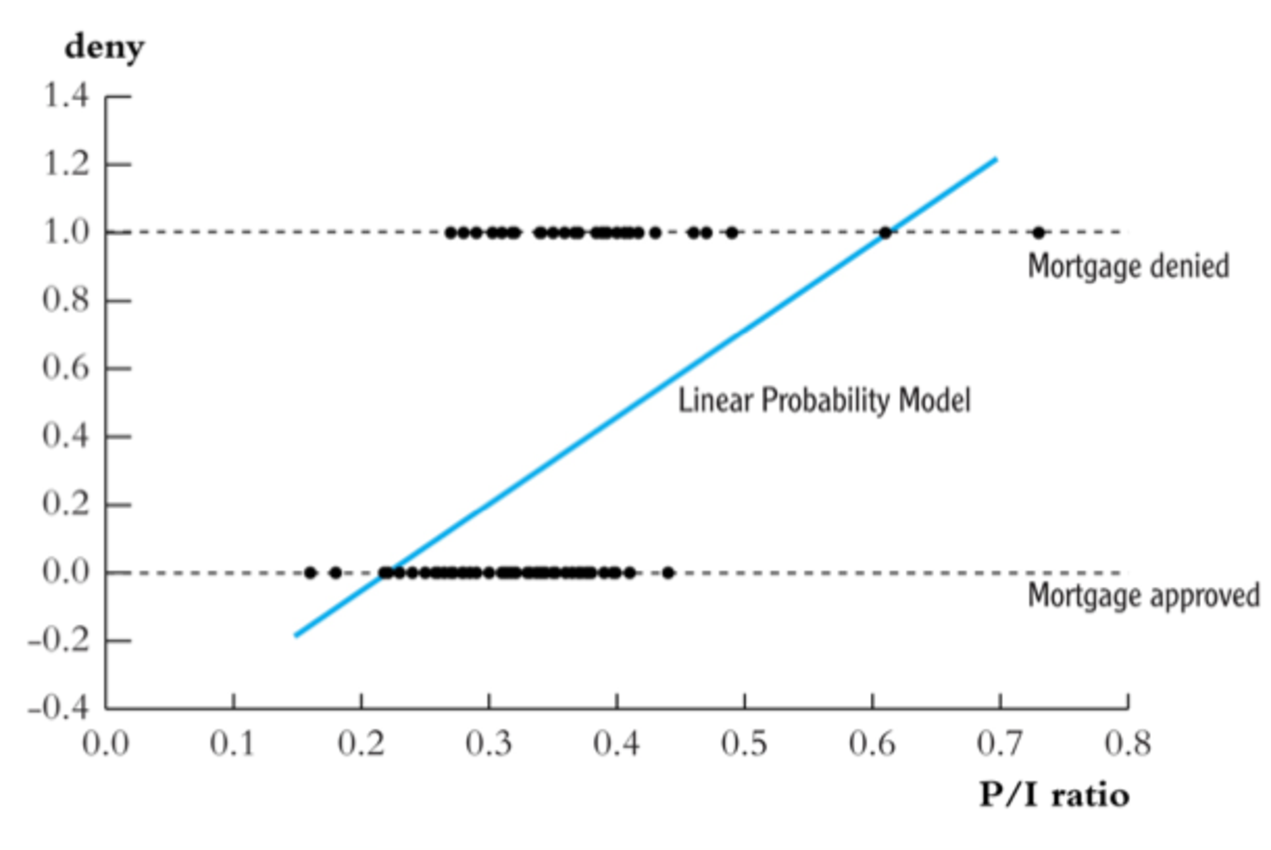
\includegraphics[width=5in]{resources/lpm.pdf}\\
\end{center}
\end{frame}

\begin{frame}{That didn't look great}
\begin{itemize}
\item Is the marginal effect $\beta_1$ actually constant or does it depend on $X$?
\item Sometimes we predict $\hat{Y} >1$ or $\hat{Y} <0$. What does that even mean? Is it still a probability?
\item Fit in the middle seems not so great -- what does $\hat{Y} = 0.5$ mean?
\end{itemize}
\end{frame}

\begin{frame}{Results}
\begin{align*}
\widehat{deny_i}= -.091 &+ .559 \cdot \text{P/I ratio}& + \alert{.177 \cdot \text{black}} \\
(0.32)&( .098) & (.025)\\
\end{align*}
Marginal Effects: 
\begin{itemize}
\item Increasing $P/I$ from $0.3 \rightarrow 0.4$ increases probabilty of denial by $5.59$ percentage points. (True at all level of $P/I$).
\item At all $P/I$ levels blacks are $17.7$ percentage points more likely to be denied.
\item But still some omitted factors.
\item True effects are likely to be \alert{nonlinear} can we add polynomials in $P/I$? Dummies for different levels? 
\end{itemize}
\end{frame}


\begin{frame}{Moving Away from LPM}
Problem with the LPM/OLS is that it requires that \alert{marginal effects are constant} or that probability can be written as linear function of parameters.
\begin{align*}
\Pr(Y=1 | X) = \beta_0 + \beta_1 X+ \varepsilon
\end{align*}
Some desirable properties:
\begin{itemize}
\item Can we restrict our predictions to $[0,1]$?
\item Can we preserve \alert{monotonicity} so that $\Pr(Y=1| X)$ is increasing in $X$ for $\beta_1 >0$?
\item Some other properties (continuity, etc.) \pause
\item Want a function $F(z): (-\infty,\infty) \rightarrow [0,1]$.
\item What function will work?
\end{itemize}
\end{frame}

\begin{frame}
\begin{center}
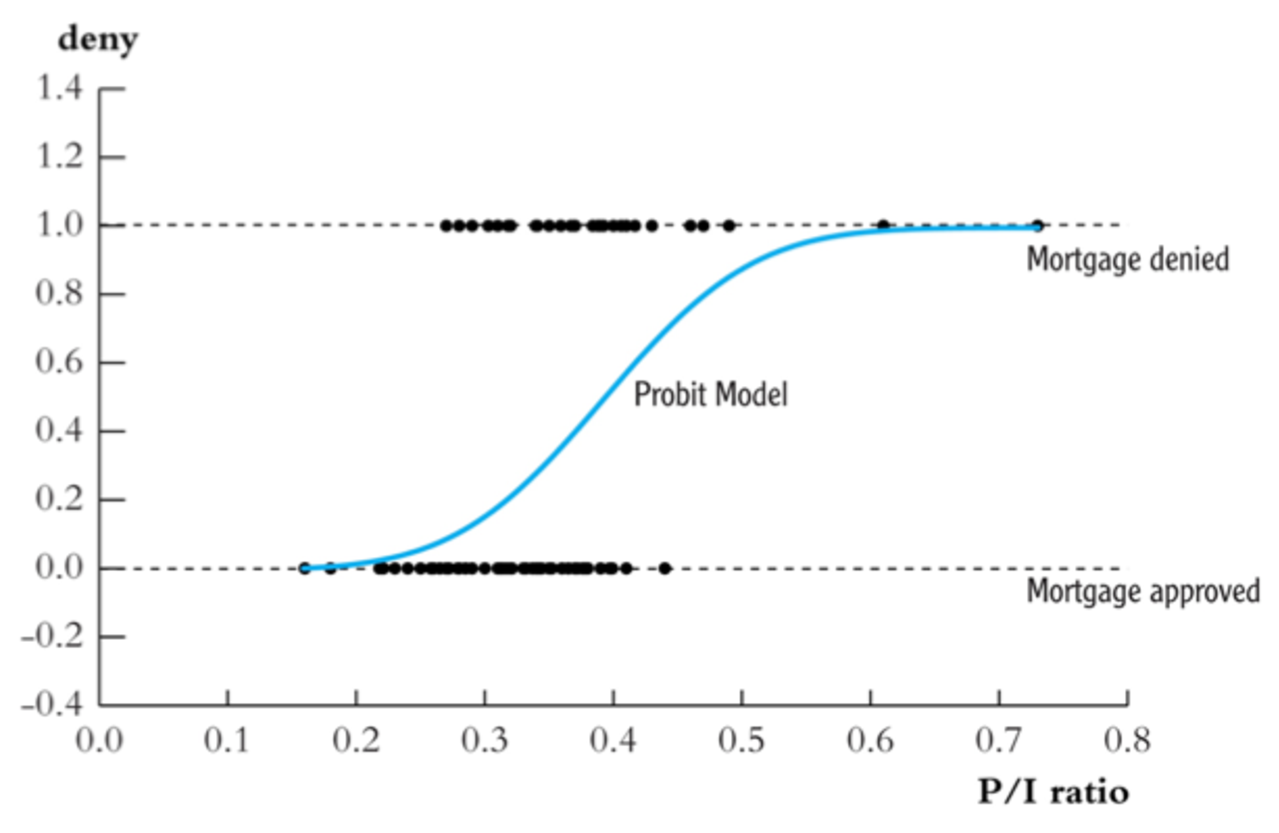
\includegraphics[width=5in]{resources/probit.pdf}
\end{center}
\end{frame}


\begin{frame}{Choosing a transformation}
\begin{align*}
\Pr(Y=1 | X) = F(\beta_0 + \beta_1 X)
\end{align*}
\begin{itemize}
\item One $F(\cdot)$ that works is $\Phi(z)$ the normal CDF. This is the \alert{probit} model.
\begin{itemize}
\item Actually any CDF would work but the normal is convenient.
\end{itemize}
\item One $F(\cdot)$ that works is $\frac{e^z}{1+ e^z}=\frac{1}{1+e^{-z}}$ the logistic function . This is the \alert{logit} model.
\item Both of these give `S'-shaped curves.
\item The LPM is $F(\cdot)$ is the \alert{identity function} (which doesn't satisfy my $[0,1]$ property).
\item This $F(\cdot)$ is often called a \alert{link function}. Why?
\end{itemize}
\end{frame}


\begin{frame}{Why use the normal CDF?}
Has some nice properties:
\begin{itemize}
\item Gives us more of the `S' shape
\item $\Pr(Y=1|X)$ is increasing in $X$ if $\beta_1>0$.
\item $\Pr(Y=1|X) \in [0,1]$ for all $X$
\item Easy to use -- you can look up or use computer for normal CDF.
\item Relatively straightforward interpretation
\begin{itemize}
\item $Z=\beta_0 + \beta_1 X$ is the $z$-value.
\item $\beta_1$ is the change in the $z$-value for a change in $X_1$.
\end{itemize}
\end{itemize}
\end{frame}


\begin{frame}{Why use the logistic CDF?}
Has some nice properties:
\begin{itemize}
\item Gives us more of the `S' shape
\item $\Pr(Y=1|X)$ is increasing in $X$ if $\beta_1>0$.
\item $\Pr(Y=1|X) \in [0,1]$ for all $X$
\item Easy to compute: $\frac{1}{1+e^{-z}}=\frac{e^{z}}{1+e^{z}}$ has analytic derivatives too.
\item Log odds interpretation
\begin{itemize}
\item $\log(\frac{p}{1-p}) = \beta_0 + \beta_1 X$
\item $\beta_1$ tells us how \alert{log odds ratio} responds to $X$.
\item $\frac{p}{1-p} \in (-\infty,\infty)$ which fixes the $[0,1]$ problem in the other direction.
\item more common in other fields (epidemiology, biostats, etc.).
\end{itemize}
\item Also has the property that $F(z) = 1-F(-z)$.
\item Similar to probit but different scale of coefficients
\item Logit/Logistic are sometimes used interchangeably but sometimes mean different things depending on the literature.
\end{itemize}
\end{frame}


\begin{frame}
\frametitle{A quick comparison}
\begin{itemize}
\item LPM prediction departs greatly from CDF long before $[0,1]$ limits.
\item We get probabilities that are too extreme even for $X\hat{\beta}$ ``in bounds''.
\item Some (MHE) argue that though $\hat{Y}$ is flawed, constant marginal effects are still OK.
\item Logit and Probit are highly similar
\end{itemize}
\begin{center}
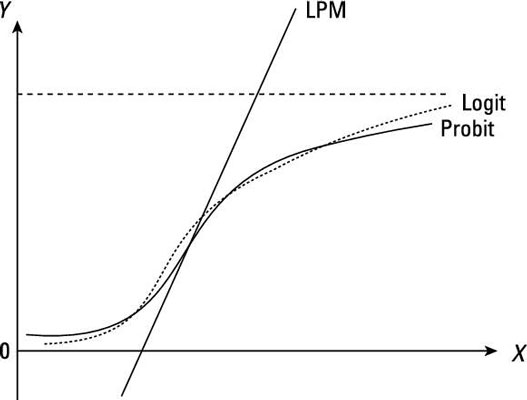
\includegraphics[width=2in]{resources/lpm-probit.jpg}
\end{center}
\end{frame}



\begin{frame}{HMDA: Results}
\begin{columns}
\begin{column}{0.4\textwidth}
\begin{center}
\scalebox{0.55}{
    
   \begin{tabular}{lccc}
      \toprule
                          &  OLS           & Probit        & Logit\\  
      \midrule
      Constant            & -0.174$^{***}$ & -2.96$^{***}$ & -5.56$^{***}$\\   
                          & (0.026)        & (0.205)       & (0.406)\\   
      Black               & 0.081$^{***}$  & 0.367$^{***}$ & 0.657$^{***}$\\   
                          & (0.017)        & (0.097)       & (0.177)\\   
      Debt/Income         & 0.471$^{***}$  & 2.58$^{***}$  & 5.03$^{***}$\\   
                          & (0.087)        & (0.546)       & (1.03)\\   
      Housing/Income      & -0.069         & -0.328        & -0.405\\   
                          & (0.096)        & (0.652)       & (1.24)\\   
      LTV: Medium         & 0.028$^{**}$   & 0.193$^{**}$  & 0.428$^{***}$\\   
                          & (0.012)        & (0.081)       & (0.158)\\   
      LTV: High           & 0.189$^{***}$  & 0.779$^{***}$ & 1.48$^{***}$\\   
                          & (0.033)        & (0.175)       & (0.309)\\   
      Consumer Credit     & 0.031$^{***}$  & 0.153$^{***}$ & 0.286$^{***}$\\   
                          & (0.004)        & (0.021)       & (0.040)\\   
      Mortgage Credit     & 0.019$^{*}$    & 0.134$^{*}$   & 0.258$^{*}$\\   
                          & (0.011)        & (0.074)       & (0.141)\\   
      Public Bad Credit   & 0.200$^{***}$  & 0.712$^{***}$ & 1.25$^{***}$\\   
                          & (0.023)        & (0.118)       & (0.205)\\   
      Denied Mortgage Ins & 0.701$^{***}$  & 2.54$^{***}$  & 4.53$^{***}$\\   
                          & (0.041)        & (0.284)       & (0.554)\\   
      \midrule
      Pseudo R$^2$        & 0.51868        & 0.26407       & 0.26586\\  
      Observations        & 2,380          & 2,380         & 2,380\\  
      \bottomrule
      \multicolumn{4}{l}{\emph{IID standard-errors in parentheses}}\\
      \multicolumn{4}{l}{\emph{Signif. Codes: ***: 0.01, **: 0.05, *: 0.1}}\\
   \end{tabular}

   }
\end{center}
\end{column}
\begin{column}{0.52\textwidth}
\begin{itemize}
    \item We cannot compare parameter estimates across specifications
    \item Rule of thumb: $\beta_{logit} \approx  1.81 \cdot \beta_{probit}$
    \item It is better to compare marginal effects $\frac{\partial \E[Y_i=1 \mid X]}{\partial x_k}$
    \item For LPM these are constant $\beta_k$, for logit/probit they depend on $X_i \beta$.
\end{itemize}
\end{column}
\end{columns}
\end{frame}


\begin{frame}
\frametitle{Index Models}
We sometimes call these single index models or threshold crossing models
\begin{align*}
Z_i = X_i \beta
\end{align*}
\begin{itemize}
\item We start with a potentially large number of regressors in $X_i$ but $X_i \beta = Z_i$ is a \alert{scalar}
\item We can just calculate $F(Z_i)$ for Logit or Probit (or some other CDF).
\item $Z_i$ is the \alert{index}. if $Z_i = X_i \beta$ we say it is a \alert{linear index} model.
\end{itemize}
\end{frame}



\begin{frame}
\frametitle{Marginal effects}
\begin{align*}
\frac{\partial \E[Y_i | X_i] }{\partial X_{ik}} = f (Z_i) \beta_k
\end{align*}
\begin{itemize}
\item The whole point was that we wanted marginal effects not to be constant
\item So where do we evaluate?
\begin{itemize}
\item Software often plugs in mean or median values for each component
\item Alternatively we can integrate over $X$ and compute:
$$
\E_{X_i}[ f (Z_i) \beta_k]
$$
\item The right thing to do is probably to plot the response surface (either probability) or change in probability over all $X$.
\end{itemize}
\end{itemize}
\end{frame}


\begin{frame}{Predicted Effects}
\begin{center}
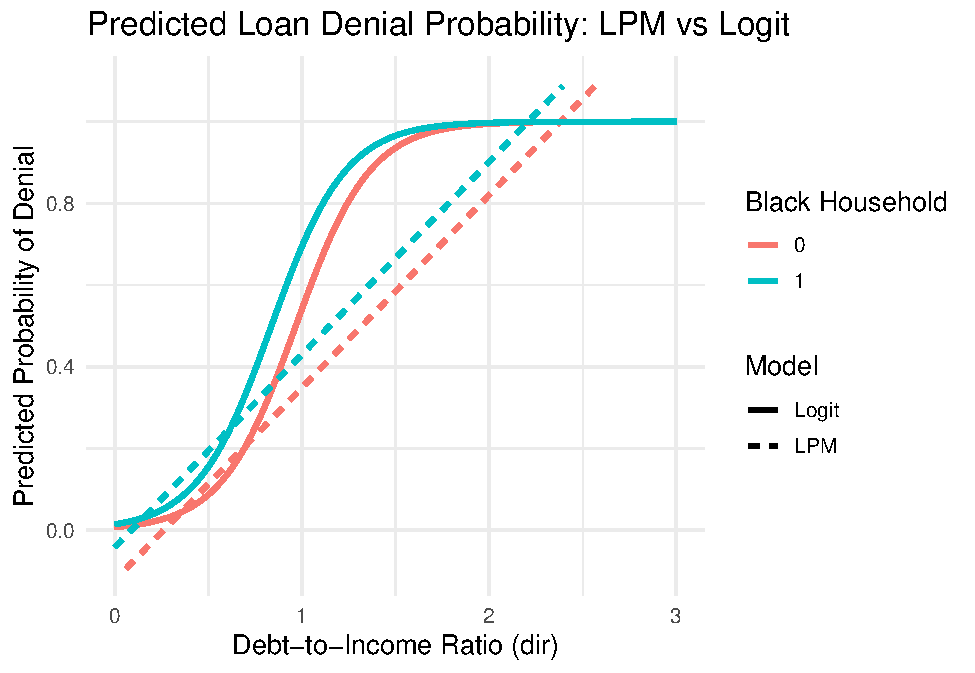
\includegraphics[height=0.9\textheight]{resources/predicted_effects.pdf}
\end{center}
\end{frame}






% \begin{frame}
% \begin{center}
% 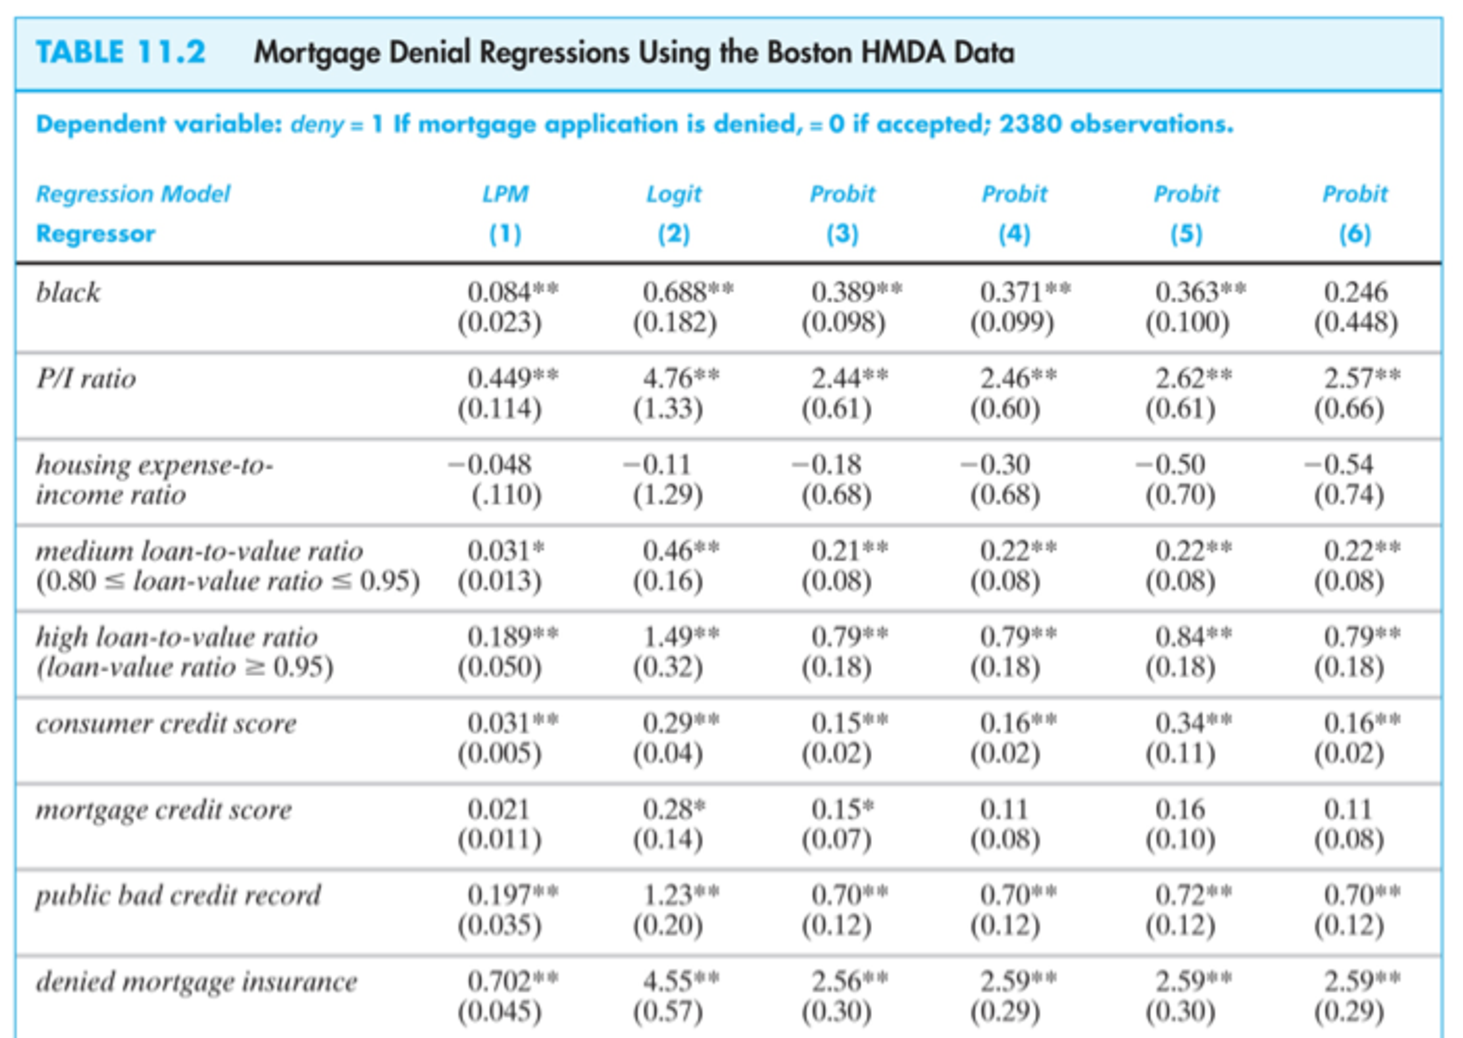
\includegraphics[width=2.5in]{resources/hmda3.pdf}\\
% 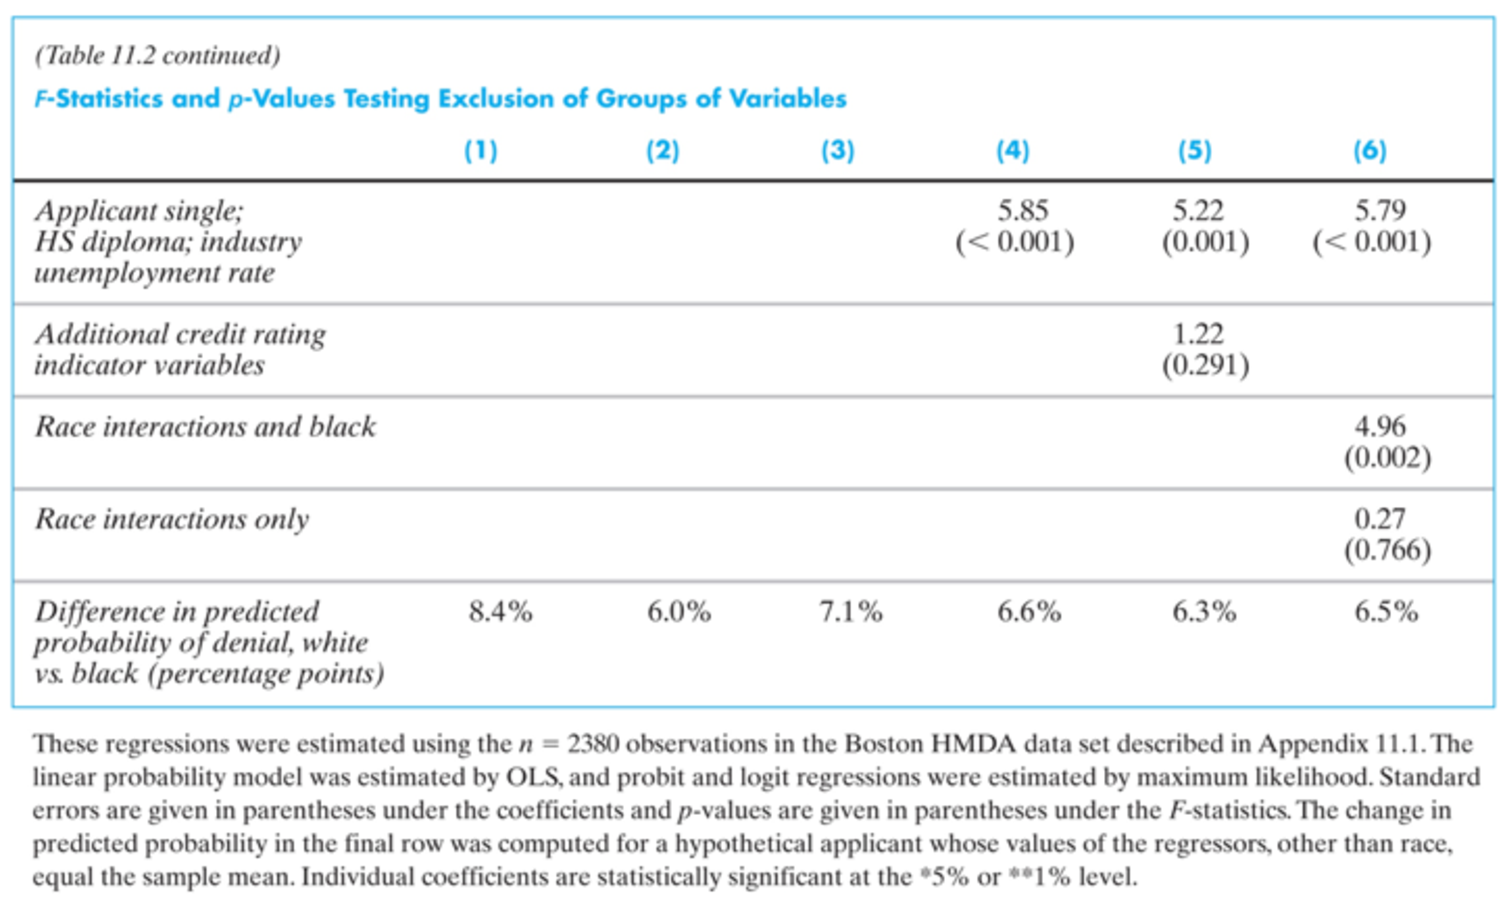
\includegraphics[width=2.5in]{resources/hmda3a.pdf}\\
% \end{center}
% \end{frame}

\begin{frame}
\frametitle{Latent Variables/ Limited Dependent Variables}
An alternative way to think about this problem is that there is a continuously distributed $Y^{*}$ that we as the econometrician don't observe.
\begin{align*}
Y_i =
\begin{cases}
1 \mbox{ if } Y^{*} >0 \\
0 \mbox{ if } Y^{*} \leq 0
\end{cases}
\end{align*}
\begin{itemize}
\item Instead we only see whether $Y^{*}$ exceeds some threshold (in this case $0$).
\item We can think about $Y^{*}$ as a \alert{latent variable}.
\item Sometimes you will see this description in the literature, everything else is the same!
\end{itemize}
\end{frame}




\begin{frame}
\frametitle{What does software do?}
\begin{itemize}
\item One temptation might be \alert{nonlinear least squares}:
\begin{align*}
\hat{\beta}^{NLLS} = \arg \min_{\beta} \sum_{i=1}^N (Y_i - \Phi(X_i \beta))^2
\end{align*}
\item Turns out this isn't what people do.
\item We can't always directly estimate using the log-odds
\begin{align*}
\log\left(\frac{p}{1-p}\right)= \beta X_i + \varepsilon_i
\end{align*}
\item The problem is that $p$ or $p(X_i)$ isn't really observed.
\end{itemize}
\end{frame}

\begin{frame}
\frametitle{What does software do?}
\begin{itemize}
\item Can construct an MLE:
\begin{align*}
\hat{\beta}^{MLE} &= \arg \max_{\beta} \prod_{i=1}^N F(Z_i)^{y_i} (1-F(Z_i))^{1-{y_i} }\\
Z_i &= \beta_0 + \beta_1 X_i
\end{align*}
\item Probit: $F(Z_i) = \Phi(Z_i)$ and its derivative (density) $f(Z_i) = \phi(Z_i)$. \\
Also is \alert{symmetric} so that $1 - F(Z_i) = F(-Z_i)$.
\item Logit: $F(Z_i) = \frac{1}{1+e^{-z}}$ and its derivative (density) $f(Z_i) = \frac{e^{-z}}{(1+e^{-z})^2}$ a more convenient property is that $\frac{f(z)}{F(z)} = 1 - F(z)$ this is called the \alert{hazard rate}.
\end{itemize}
\end{frame}

\begin{frame}
\frametitle{A probit trick}
Let $q_i = 2 y_i -1$
\begin{align*}
F(q_i \cdot Z_i) = 
\begin{cases}
F(Z_i)  &\mbox{ when } y_i=1 \\
F(-Z_i) = 1-F(Z_i)& \mbox{ when } y_i=0
\end{cases}
\end{align*}
So that 
\begin{align*}
\ell(y_1,\ldots, y_n | \beta) = \sum_{i=1}^N \ln F(q_i \cdot Z_i) 
\end{align*}
\end{frame}


\begin{frame}
\frametitle{FOC of Log-Likelihood}
\begin{align*}
\ell(y_1,\ldots,y_n | \beta) &= \sum_{i=1}^N y_i \ln F(Z_i) + (1-y_i) \ln(1- F(Z_i)) \\
\frac{\partial l }{\partial \beta} &= \sum_{i=1}^N \frac{y_i}{ F(Z_i)} \frac{ d F}{d \beta}(Z_i) - \frac{1-y_i}{1-F(Z_i)}  \frac{ d F}{d \beta} (Z_i)\\
 &= \sum_{i=1}^N \frac{y_i \cdot f(Z_i) }{ F(Z_i)} \frac{ d Z_i}{d \beta} -  \sum_{i=1}^N \frac{(1-y_i)\cdot f(Z_i) }{1-F(Z_i)} \frac{ d Z_i}{d \beta} \\
 &= \sum_{i=1}^N  \left[ \frac{y_i \cdot f(Z_i) }{ F(Z_i)} X_i -  \frac{(1-y_i)\cdot f(Z_i) }{1-F(Z_i)} X_i \right] 
\end{align*}
\end{frame}

\begin{frame}
\frametitle{FOC of Log-Likelihood (Logit)}
This is the \alert{score} of the log-likelihood:
\begin{align*}
\frac{\partial l }{\partial \beta} = \nabla_{\beta} \cdot \ell(\symbf{y}; \beta) &=  \sum_{i=1}^N  \left[ y_i \frac{ f(Z_i) }{ F(Z_i)}  -  (1-y_i) \frac{f(Z_i) }{1-F(Z_i)} \right]  \cdot X_i 
\end{align*}
It is technically also a \alert{moment condition}. It is easy for the logit
\begin{align*}
 \nabla_{\beta} \cdot \ell(\symbf{y}; \beta) &=  \sum_{i=1}^N  \left[ y_i (1-F(Z_i)) -  (1-y_i) F(Z_i) \right] \cdot X_i \\
 &=  \sum_{i=1}^N  \underbrace{\left[ y_i - F(Z_i) \right]}_{\varepsilon_i} \cdot X_i 
\end{align*}
This comes from the hazard rate.
\end{frame}

\begin{frame}
\frametitle{FOC of Log-Likelihood (Probit)}
This is the \alert{score} of the log-likelihood:
\begin{align*}
\frac{\partial l }{\partial \beta} = \nabla_{\beta} \cdot \ell(\symbf{y}; \beta) &=  \sum_{i=1}^N  \left[ y_i \frac{ f(Z_i) }{ F(Z_i)}  -  (1-y_i) \frac{f(Z_i) }{1-F(Z_i)} \right] \cdot X_i  \\
 &=  \sum_{y_i=1}  \frac{\phi(Z_i) }{ \Phi(Z_i)} X_i +\sum_{y_i=0} \frac{-\phi(Z_i) }{1-\Phi(Z_i)} X_i
\end{align*}
Using the $q_i = 2 y_i -1$ trick
\begin{align*}
\nabla_{\beta} \cdot \ell(\symbf{y}; \beta)= \sum_{i=1}^N \underbrace{\frac{ q_i \phi(q_i Z_i)}{\Phi(Z_i)}}_{\lambda_i} X_i
\end{align*}
\end{frame}


\begin{frame}
\frametitle{The Hessian Matrix}
We could also take second derivatives to get the \alert{Hessian} matrix:
\begin{align*}
\frac{\partial l^2 }{\partial \beta \partial \beta'} = - \sum_{i=1}^N   y_i \frac{ f(Z_i)  f(Z_i) - f'(Z_i) F(Z_i) }{ F(Z_i)^2}  X_i X_i' \\
+  \sum_{i=1}^N   (1-y_i) \frac{f(Z_i)f(Z_i) - f'(Z_i)(1-F(Z_i))}{(1-F(Z_i))^2}  X_i X_i'
\end{align*}
This is a $K\times K$ matrix where $K$ is the dimension of $X$ or $\beta$.
\end{frame}



\begin{frame}
\frametitle{The Hessian Matrix (Logit)}
For the logit this is even easier (use the simplified logit score):
\begin{align*}
\frac{\partial l^2 }{\partial \beta \partial \beta'}  &= - \sum_{i=1}^N f(Z_i) X_i X_i' \\
&= - \sum_{i=1}^N F(Z_i) (1- F(Z_i)) X_i X_i'
\end{align*}
This is \alert{negative semi definite}
\end{frame}

\begin{frame}
\frametitle{The Hessian Matrix (Probit)}
Recall
\begin{align*}
\nabla_{\beta} \cdot \ell(\symbf{y}; \beta)= \sum_{i=1}^N \underbrace{\frac{ q_i \phi(q_i Z_i)}{\Phi(Z_i)}}_{\lambda_i} X_i
\end{align*}
Take another derivative and recall $\phi'(z_i) = - z_i \phi(z_i)$
\begin{align*}
\nabla_{\beta}^2 \cdot \ell(\symbf{y}; \beta)&= \sum_{i=1}^N \frac{q_i \phi'(q_i Z_i) \Phi(z_i) - q_i \phi(z_i)^2}{\Phi(z_i)^2}  X_i X_i' \\
&= - \lambda_i( z_i + \lambda_i) \cdot X_i X_i'
\end{align*}
Hard to show but this is \alert{negative definite} too.
\end{frame}


% \begin{frame}
% \frametitle{Estimation}
% \begin{itemize} 
% \item We can try to find the values of $\beta$ which make the average score $=0$ (the FOC).
% \item But no closed form solution!
% \item Recall Taylor's Rule:
% \end{itemize}
% \begin{align*}
% f(x + \Delta x) =  f(x_0) + f'(x_0) \Delta x + \frac{1}{2} f''(x_0) (\Delta x)^2
% \end{align*}
% Goal is to find the case where $f'(x) \approx 0$ so take derivative w.r.t $\Delta x$:
% \begin{align*}
% \frac{d}{d \Delta x} \left[  f(x_0) + f'(x_0) \Delta x + \frac{1}{2} f''(x_0) (\Delta x)^2 \right] = f'(x_0) +  f''(x_0) (\Delta x) = 0
% \end{align*}
% Solve for $\Delta x$
% \begin{align*}
% \Delta x  = - f'(x_0) / f''(x_0)
% \end{align*}
% \end{frame}



% \begin{frame}
% \frametitle{Estimation}
% \begin{itemize} 
% \item In multiple dimensions this becomes:
% \begin{align*}
% x_{n+1} = x_{n} - \alpha \cdot \left[\symbf{H}_f (x_n) \right]^{-1} \nabla f(x_n)
% \end{align*}
% \item $\symbf{H}_f (x_n)$ is the \alert{Hessian} Matrix. $ \nabla f(x_n)$ is the \alert{gradient}.
% \item $\alpha \in [0,1]$ is a parameter that determines \alert{step size}
% \item Idea is that we approximate the likelihood with a quadratic function and minimize that (because we know how to solve those).
% \item Each step we update our quadratic approximation.
% \item If problem is \alert{convex} this will always converge (and quickly)
% \item Most software ``cheats'' and doesn't compute $\left[\symbf{H}_f (x_n) \right]^{-1}$ but uses tricks to update on the fly (BFGS, Broyden, DFP, SR1). Mostly you see these options in your software.
% \end{itemize}
% \end{frame}



\begin{frame}
\frametitle{Inference}
\begin{itemize} 
\item If we have the Hessian Matrix, inference is straightforward.
\item $\symbf{H}_f(\hat{\beta}^{MLE})$ tells us about the \alert{curvature} of the log-likelihood around the maximum.
\begin{itemize}
\item Function is flat $\rightarrow$ not very precise estimates of parameters
\item Function is steep $\rightarrow$  precise estimates of parameters
\end{itemize}
\item Construct \alert{Fisher Information} $I(\hat{\beta}^{MLE}) = -\E[\symbf{H}_f(\hat{\beta}^{MLE})]$ where expectation is over the data.
\begin{itemize}
\item Logit does not depend on $y_i$ so $\E[\symbf{H}_f(\hat{\beta}^{MLE})]=\symbf{H}_f(\hat{\beta}^{MLE})$.
\item Probit does depend on $y_i$ so $\E[\symbf{H}_f(\hat{\beta}^{MLE})]\neq \symbf{H}_f(\hat{\beta}^{MLE})$.
\end{itemize}
\item Inverse Fisher information $-\E[\symbf{H}_f(\hat{\beta}^{MLE})]^{-1}$ is an estimate of the variance covariance matrix for $\hat{\beta}$.
\item $\sqrt{\text{diag}[\E[-\symbf{H}_f(\hat{\beta}^{MLE})]^{-1}]}$ is an estimate for $SE(\hat{\beta})$.
\end{itemize}
\end{frame}

\begin{frame}
\frametitle{Goodness of Fit \#1: Pseudo $R^2$}
How well does the model fit the data?
\begin{itemize} 
\item No $R^2$ measure (why not?).
\item Well we have likelihood units so average likelihood tells us something but is hard to interpret.
\item $\rho = 1- \frac{\ell(\hat{\beta}^{MLE})}{\ell(\beta_0)}$ where $\ell(\beta_0)$ is the likelihood of a model with just a constant (unconditional probability of success).
\begin{itemize}
\item If we don't do any better than unconditional mean then $\rho=0$.
\item Won't ever get all of the way to $\rho =1$.
\end{itemize}
\end{itemize}
\end{frame}

\begin{frame}
\frametitle{Goodness of Fit \#2: Confusion Matrix }
\begin{itemize} 
\item Machine learning likes to think about this problem more like \alert{classification} then regression.
\item A caution: these are \alert{regression} models not \alert{classification} models.
\item Predict either $\hat{y}_i = 1$ or $\hat{y}_i = 0$ for each observation.
\item Predict $\hat{y}_i =1$ if $\Pr(y_i = 1 | X_i =x) \geq0.5$ or $F(X_i \hat{\beta}) > 0.5$.
\item Imagine for cells Prediction: $\{Success, Failure\}$, Outcome $\{Success, Failure\}$
\item Can construct this using the R package \texttt{caret} and command \texttt{caret}.
\end{itemize}
\end{frame}


\begin{frame}{ROC Curve/ AOC}
\begin{center}
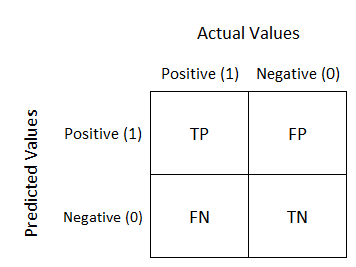
\includegraphics[width=3in]{resources/confusion.png}\\
\end{center}
\end{frame}



\begin{frame}{ROC Curve/ AOC}
\begin{center}
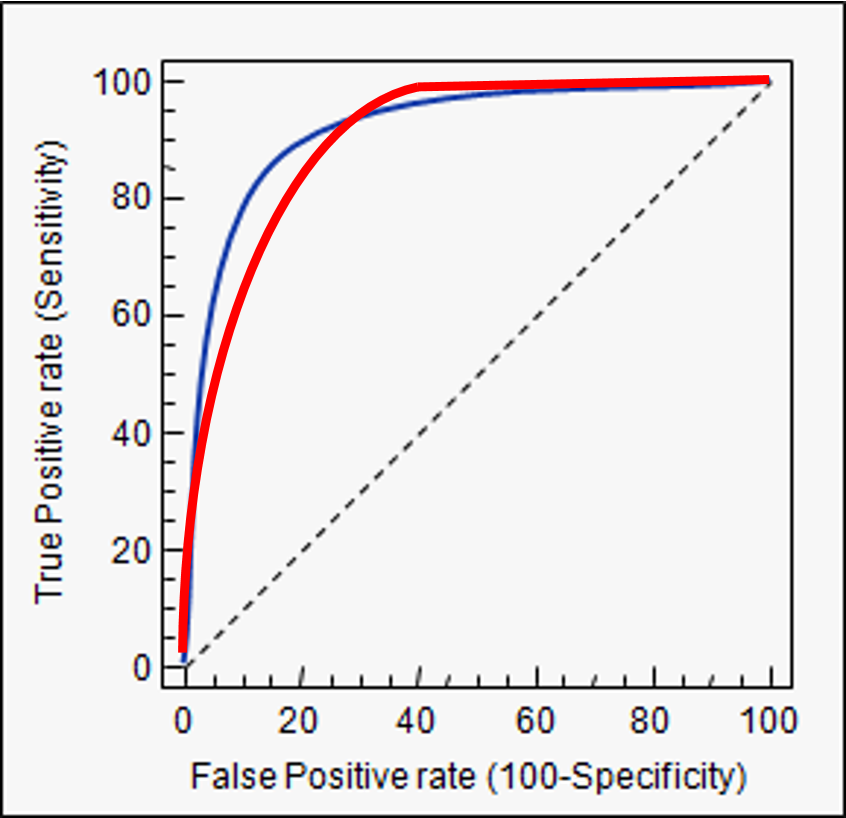
\includegraphics[width=2.5in]{resources/roc_curve.png}\\
\end{center}
\begin{itemize}
\item At each predicted probability calculate both \alert{True Positive Rate} and \alert{False Positive Rate}.
\item AOC is area under the curve
\end{itemize}
\end{frame}


\section{Thanks!}

\end{document}